\chapter{System's architecture}

\section{Components}
For this project, 3 main components are required (fig. \ref{00fig}):
\begin{enumerate}
	\item \textbf{IP-core Manager}:it's the main element of this architecture and its main goal is to handle the complexity of this system. It has to provide the correct exchange of data between the target IP-core and the CPU. Moreover it has to handle the interrupt service routine.
	\item \textbf{Data Buffer}:it's a dual port buffer that stores the data coming both from the CPU and the selected IP-core. It also enable the communication of the desired transaction from the CPU to the IP-core Manager by means of the $ row0 $ which is always read from the IP-core Manager
	\item \textbf{IP-core}:a core that perform a specific task or function.
\end{enumerate}
\section{Interfaces}

A multi IP-core system requires a IP core manager to handle the complexity of this system.
Main tasks of the IP Manager are the correct exchange of data between the target IP and the CPU. Another critical task is the interrupt handling. Figure \ref{00fig} shows the overall architecture of the whole system adopted.\\
	
	As shown in the figure \ref{00fig}, the IP manager indirectly communicates with the CPU through a dual port data buffer. This buffer has a standard interface and it is used to redirect data to/from the IP core selected.
	Whenever the CPU wants to start a transaction, it has to write some control bits (explained in section \ref{transaction}) at address 0 ($ row0 $) of the data buffer.
	The data in this address is always read from the IP Manager to speed-up the routing process whenever a new transaction begins.\\
\subsection{Data Buffer interface}\label{bufinter}
This data buffer has a standard interface.
The signals for this components (whether they come from the CPU or from from the IP core Manager of from both of them) has the following function: 
\begin{itemize}
	\item \textbf{data}: input/output port, used for transferring data from/to the CPU to/from the buffer. 
	\item \textbf{add}: input port, used for selecting the right row within the buffer to write/read data. 
	\item \textbf{w\_enable}: input port, must be asserted in order to enable write operation. 
		\item \textbf{w\_enable}: input port, must be asserted in order to enable read operation.  
		\item \textbf{generic\_enable}: input port, must be asserted in order to start any operation on that port. 
		\item \textbf{reset}: input port, it brings the buffer to the reset state. 
		\item \textbf{row\_0}: output port, it reflects any change in the row 0 of the buffer. 
\end{itemize}
\subsection{IP core interface} \label{IPinter}
	As for a generic $ x $ IP core interface, we have the following signals:
	\begin{itemize}
	\item \textbf{data\_in\_IPs(x)}:data from the $ x $ IP-core to the CPU/Data buffer.
\item \textbf{data\_out\_IPs(x)}:data to the $ x $ IP-core from the CPU/Data buffer.
\item \textbf{add\_IPs(x)}:address from the $ x $ IP-core to the Data buffer.
\item \textbf{W\_enable\_IPs(x)}: when the $ x $ IP-core wants to write to the buffer
\item \textbf{R\_enable\_IPs(x)}: when the $ x $ IP-core wants to read from the buffer
\item \textbf{Generic\_en\_IPs(x)}: when the $ x $ IP-core wants to communicate with the buffer	
\item \textbf{enable\_IPs(x)}: when the CPU wants to communicate with the $ x $ IP-core
\item \textbf{ack\_IPs(x)}: the IP-core manager sent this signal to the $ x $ IP-core to tell it that its interrupt request will be served
\item \textbf{interrupt\_IPs(x)}: when the $ x $ IP-core raises an interrupt request
\end{itemize}
	\begin{figure}[h]
		\centering
		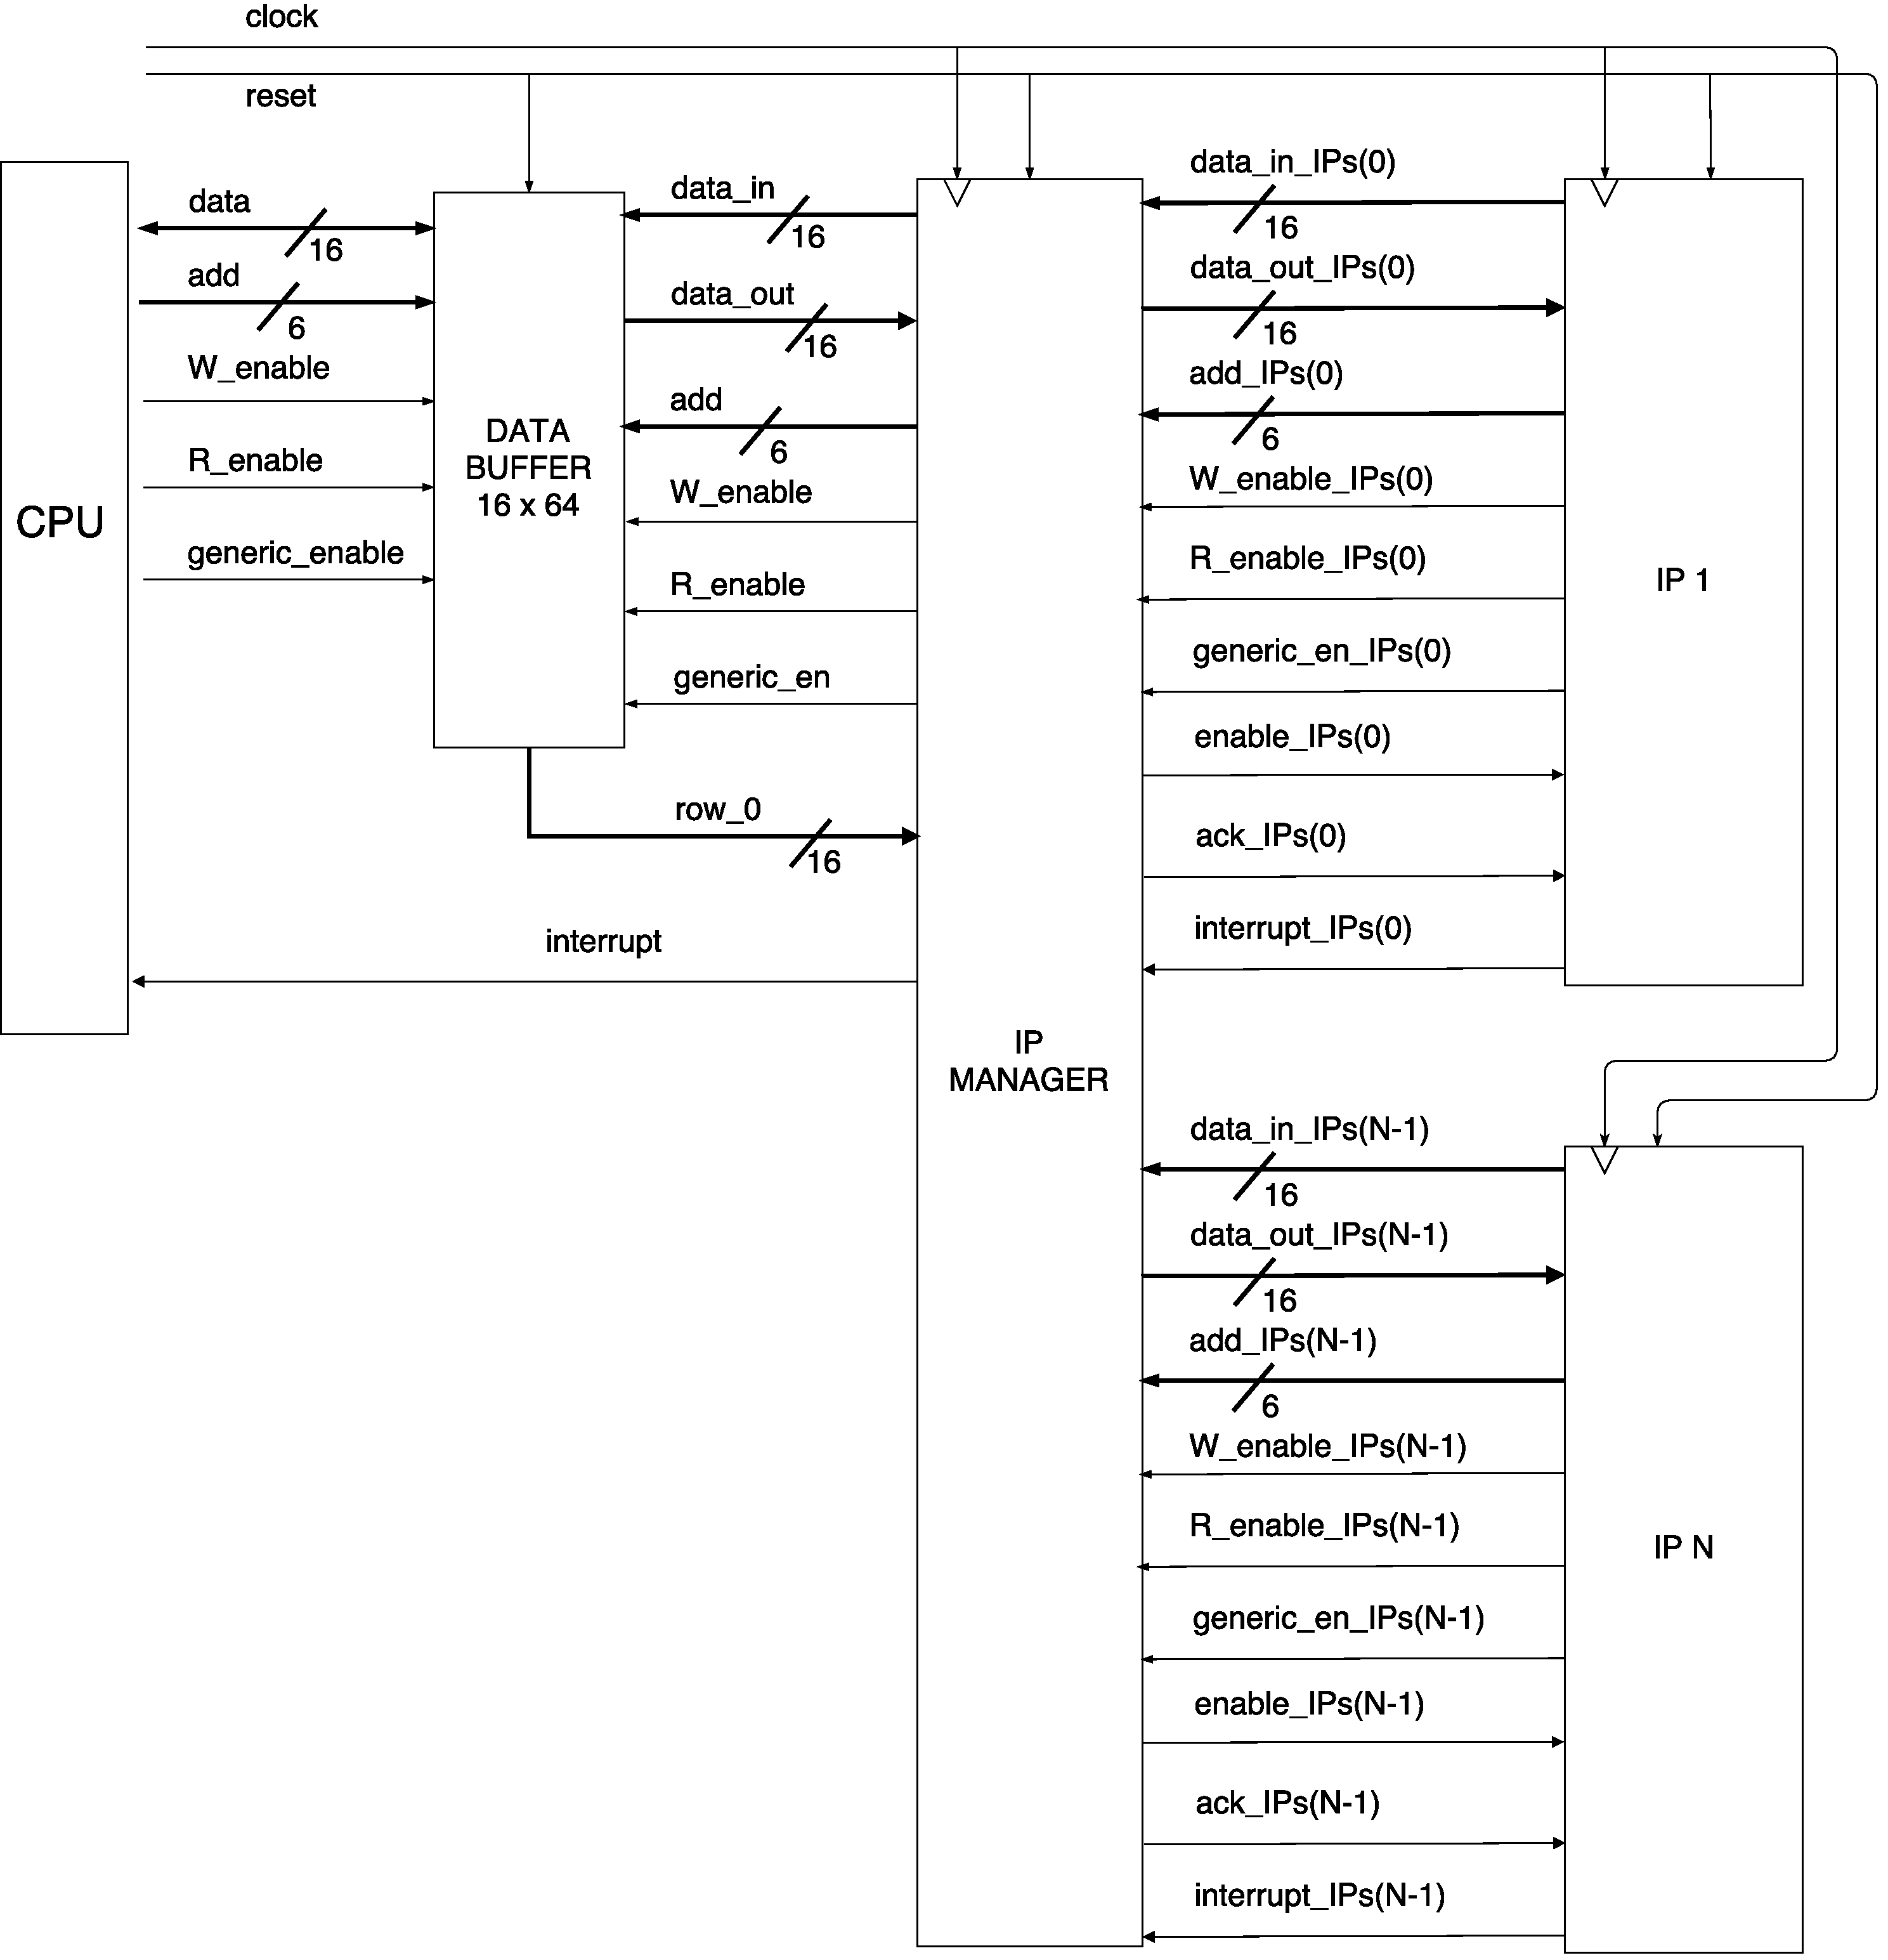
\includegraphics[width=0.95\textwidth]{chapters/figures/Interface.pdf}  
		\caption{System architecture}
		\label{00fig}
	\end{figure}
\clearpage
\newpage
\section{CPU Control bits } \label{transaction}

	When the CPU wants to start a transaction, it has to write a data packet with the following structure\\
	\begin{center}
	\begin{tabular}{ | l | l |  l | l | }
		
		15  \qquad  \qquad 14 & 13 & 12 & 11 \qquad \qquad 0 \\ \hline
		UNUSED & INT & B/E & IP ADDR\\ \hline
		
		
		\hline
	\end{tabular}
\end{center}

\bigskip
\begin{center}
	\begin{tabular}{ | c | p{7 cm} |  l |}
		\hline
		Bit(s) & Purpose & Value(s)  \\ \hline
		Bit 15 & unused  & unused 
		\\ \hline
		Bit 14 & unused  & unused\\
		\hline
		Bit 13 & Interrupt ACK from the CPU   & Normal = 0, Interrupt  =  1
		\\ \hline
		
		Bit 12 & Signals the begin/end of a transaction & Begin  = 1, End = 0 
		\\ \hline
			
		
			
		Bit 11-0 & The physical address of the target IP &
		From 0 up to N-1  \\
		
		
		
		\hline
	\end{tabular}
\end{center}
For a better understanding of the transaction mechanism, please see chapter \ref{usecase}.
